\documentclass[11pt]{article}
\usepackage{graphicx, xcolor}
\usepackage{wrapfig}
\usepackage[section]{placeins}

\title{{Intermediate Report}}
\date{}
\author{team\_we\_got\_this}
\begin{document}
\maketitle

\section{Introduction}

\section{Project Description}

\subsection{Overview of our Simulation}

	Our group proposes to build a four junction roundabout with multiple lanes to allow overtaking the junctions and policies we introduce will be loosely based on exiting roundabouts in and around London. Originally our design included traffic lights but within two weeks we had working traffic lights on our test simulation. Hence, it was decided that it would more challenging to build a roundabout without traffic lights, as our cars would then need to be intelligent enough to know when to give way to other cars already on the roundabout. We aim to also allow users to change the probability of cars coming from each junction in order to accurately measure real life scenarios. For example, if there was a heavy flow of cars from one junction, this will stop cars from the junction to the left of it entering the roundabout as they will have to give way.\textcolor{red}{If there is space show this in a picture}
	
	If we could succeed in implementing the giveway policy we could then create our own scenario, introduce
    traffic lights to analyse network flow and try to make improvements. We will then analyse how many cars enter the roundabout from each junction per minute. Our system would give users control of the time duration of the lights so that we could allow lights to be green for a longer duration at junction where the traffic flow is heavy. As an optional attribute to our system we would like to implement traffic lights which are dynamic and will change colour based on the number of cars passing through instead of time elapsed. \\


\begin{tabular}{ | l | c | r | }
	 \hline
	\multicolumn{3}{|c|}{Project Timetable}  \\ \hline
	Date & Description of Implementation & Status \\ \hline
	22/01/15 & Basic model with moving cars &  Achieved \\ \hline
	29/01/15 & Collision detection and avoidance & Achieved \\ \hline
	16/02/15 & Working Basic Cellular Automation model & Pending \\ \hline
	16/02/15 & Roundabout & Pending \\ \hline
	16/02/15 & Multi-lane roundabout & Pending \\ \hline
	
\end{tabular}
\subsection{Design Approach 1:Cellular Automation}
Two members of the group felt that using a cell based approach would be most effective. The had to separate ideas and these will be discussed in the section below. 
	


\noindent {\bf Anton's Model}
\begin{itemize}
	\item We explored the possibility of building our entire system in Actionscript. It was initially proposed to build it on a hexagon grid, using coordinates to track the position of cars on the grid.The hexagon grid was thought to better suit the needs of our roundabout. \textcolor{red}{why did this not work?} 
	\item pros of Anton's model: Anton was the first to have a traffic light which had green for different directions and have cars which could respond to this, i.e. if a light was green for straight ahead only and the car at the light wanted to turn left, the car would not go. The cars could not respond to other cars on the road and hence if a car was travelling at a faster speed than the car in front of it, it would go through it. 
\end{itemize}


\noindent{\bf Zaki's model:}
\begin{itemize}
	\item Explan where celluar automation came from
	\item Explain how we would use it
\end{itemize}
\subsection{Design Approach 2: Using Equations}

{\bf Nur's Model:}\\\\
This model was the first working model the group created. It is built by recolouring pixels every 30 milliseconds to show movement of the cars across the map. 

%
%%\begin{figure}{H}
%	\begin{center}
%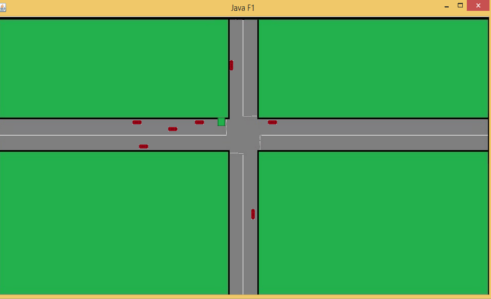
\includegraphics[width=0.50\textwidth]{ScreenShotNurSim.pdf}
%\center{A screen-shot of our first simulation}
%\end{center}
%
%%\end{figure}
\FloatBarrier
\begin{figure}[h]
	\centering
	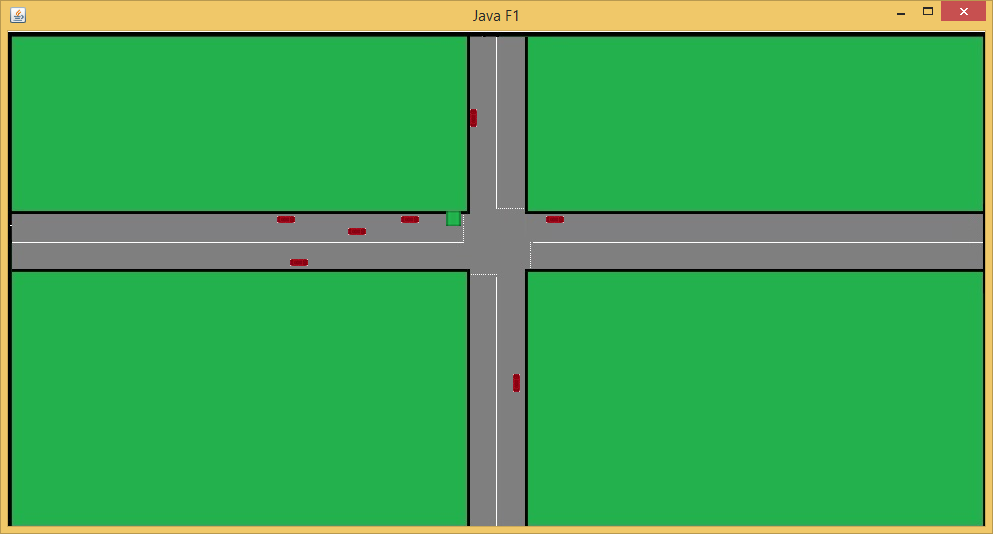
\includegraphics[width=0.45\textwidth]{ScreenShotNurSim}
	\caption{Screenshot of our first working model}
	
\end{figure}

We had this working model very quickly and a clear understanding of how we could adapt to fit the needs of our roundabout but we questions whether it would be dynamic enough to adapt to our growing plans. In this system the map is on a coordinate system and a car travelling at say $30 m/s$ from west to east would increase its x-coordinate by 30 in the next time frame and similarly for other movements. However this would suit our current simple crossroad but as our system developed in to a multi-lane roundabout this naive approach would begin to hold us back.

Originally this model had an issue with collisions as our cars did not know of the other existence. This problem was fixed by each car first checking if its new coordinates will intersect with the coordinates of another car already on the map. If it does intersect then car will try to change into the right lane. If the right lane is occupied or if it is already in the right lane the car will stay where it is,following the car in front. Our cars also only overtake from the outside and know not to overtake by crossing into the lane for traffic flowing in the opposite direction. We would like to the adapt the system so that a car and can alert the car in front that it is moving too slow and have the other car receive this message and react according just like in real life. This has the possibility to be extended into speed restriction for each lane, i.e. the maximum speed in the left lane being $30m/s$ whilst the right lane could be the fast lane with a maximum speed of $60m/s$\\

\noindent{\bf{Kim's approach:}}\\\\
The final approach we consider was a continuous model in which our map was represented by several intersecting lines (see figure 2 below). Although this approach would allow us to accurately calculate where each car is at any time , decided that the implementation would be unnecessarily time-consuming.  

\FloatBarrier
\begin{figure}
	\centering
	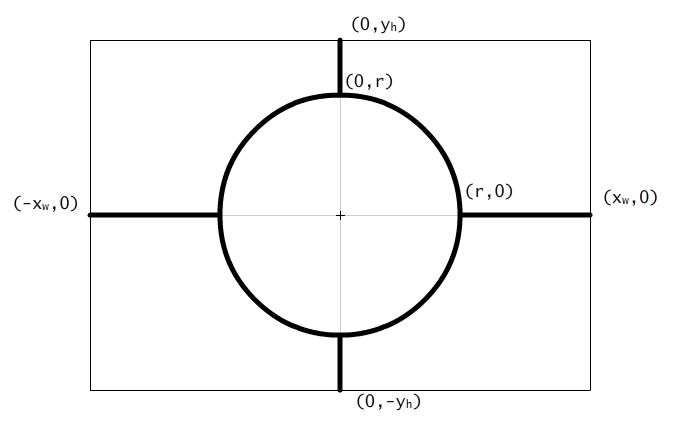
\includegraphics[width=0.45\textwidth]{KimsModel}
	\caption{Sample graph for Our Continuous Model}
\end{figure}

\section{Project Organisation}
\begin{itemize}
\item meetings twice a week and use of dropbox to share files which we can't put on github. 
\item Roles:\\
Rochelle team coordinator and administrator. \\
Nur - Software developer\\
Zaki - Software developer \\
Anton - Software developer \\
Kim - Graphics coordinator/ assistant software developer  
\end{itemize}
\begin{itemize}

\item We will use Java as are back-end but we are considering writing our GUI in action-script because two members of the team are familiar with it. 
\item In the peer assessment we plan to give everyone equal points as we all have pre-defined and necessary roles in the project. 
\item In the beginning we had issue with the meetings slots as this is still on going. We try to compromise on smaller issue and then just vote on any large issue.  

\end{itemize}

\end{document}